\documentclass[11pt,letterpaper]{article}
\PassOptionsToPackage{hyphens}{url}
\usepackage[margin=.83in,top=.8in,bottom=.8in,headheight=15pt]{geometry}
\usepackage[T1]{fontenc}
\usepackage{lmodern,amsmath,amssymb,mathtools,bm,booktabs,array,graphicx,tikz}
\usetikzlibrary{arrows.meta,positioning,calc,decorations.pathreplacing,patterns}
\definecolor{ink}{HTML}{17344D}\definecolor{accent}{HTML}{087E8B}\definecolor{pale}{HTML}{EDF5F5}\definecolor{gold}{HTML}{AD6B19}
\providecommand{\dd}{\,\mathrm{d}}\providecommand{\R}{\mathbb{R}}
\providecommand{\E}{\mathbb{E}}\providecommand{\Var}{\operatorname{Var}}
\providecommand{\Cov}{\operatorname{Cov}}\providecommand{\diag}{\operatorname{diag}}
\providecommand{\norm}[1]{\left\lVert#1\right\rVert}
\providecommand{\abs}[1]{\left|#1\right|}
\usepackage{microtype,hyperref,fancyhdr,enumitem,amsthm,sectsty,needspace}
\allsectionsfont{\raggedright}
\hypersetup{colorlinks=true,linkcolor=ink,urlcolor=accent,pdfauthor={Zan Ahmad},pdftitle={Calibrating a flow law and constructing a classifier / Lecture notes}}
\setlength{\parindent}{0pt}\setlength{\parskip}{6pt}\linespread{1.07}
\setlist{itemsep=3pt,topsep=4pt,leftmargin=*}
\emergencystretch=2em\clubpenalty=10000\widowpenalty=10000
\pagestyle{fancy}\fancyhf{}\fancyhead[L]{\small Mathematical Cardiology}\fancyhead[R]{\small Lecture 8}
\fancyfoot[L]{\footnotesize Zan Ahmad}\fancyfoot[R]{\footnotesize\thepage}\renewcommand{\headrulewidth}{.3pt}
\newtheorem{proposition}{Proposition}\newtheorem{theorem}{Theorem}\newtheorem{lemma}{Lemma}
\theoremstyle{definition}\newtheorem{definition}{Definition}\newtheorem{example}{Example}
\numberwithin{equation}{section}
\begin{document}
{\small\scshape Mathematical Cardiology\hfill Lecture 8}\par\medskip
{\raggedright\hyphenpenalty=10000\exhyphenpenalty=10000\LARGE\bfseries\color{ink} Calibrating a flow law and constructing a classifier\par}\medskip
{\small Lecture notes}\par\bigskip
A physical relation can be known in form while containing an unknown parameter. In $Q=G\Delta P$, for example, a measured flow can tell us something about conductance $G$. The same observation cannot also serve as an independent test of the parameter it selected. We shall first derive a calibration rule, then construct a classifier whose fitted quantities are equally explicit. In both cases the algebra will reveal what the data can determine and what must remain outside the fitted calculation.

\section{A passive law with an unknown coefficient}
\hypertarget{note-a-passive-law-with-an-unknown-coefficient}{}\label{note:a-passive-law-with-an-unknown-coefficient}
{\small \href{slides.html\#frame=a-parameter-inside-a-physical-relation-figure\&step=1}{Slides for this section}}\par
Let $x_i$ be the pressure difference in experiment $i$, measured in mmHg, and let $y_i$ be the observed flow in L/min. The proposed law predicts $\widehat y_i=Gx_i$, where $G$ has units $\mathrm{L/(min\,mmHg)}$. Its resistance is $R=1/G$ when $G>0$. Choosing a line through the origin is a physical assumption: equal boundary pressures produce zero passive flow. An offset would require a different model, perhaps one for measurement bias or an active pressure source.

Define the residual as prediction minus observation, $r_i(G)=Gx_i-y_i$. Positive and negative residuals can cancel even when both are large. We therefore consider
\begin{equation}S(G)=\sum_{i\in\mathcal T}(Gx_i-y_i)^2,\end{equation}
where $\mathcal T$ contains training observations only. Each term and the sum have units $(\mathrm{L/min})^2$. Squaring is a choice of discrepancy measure; it gives a larger penalty to a large error than to several smaller errors with the same total absolute size. Neither this choice nor the resulting minimizer proves that the passive law is the right mechanism.
\begin{center}\begin{minipage}{.98\linewidth}\centering
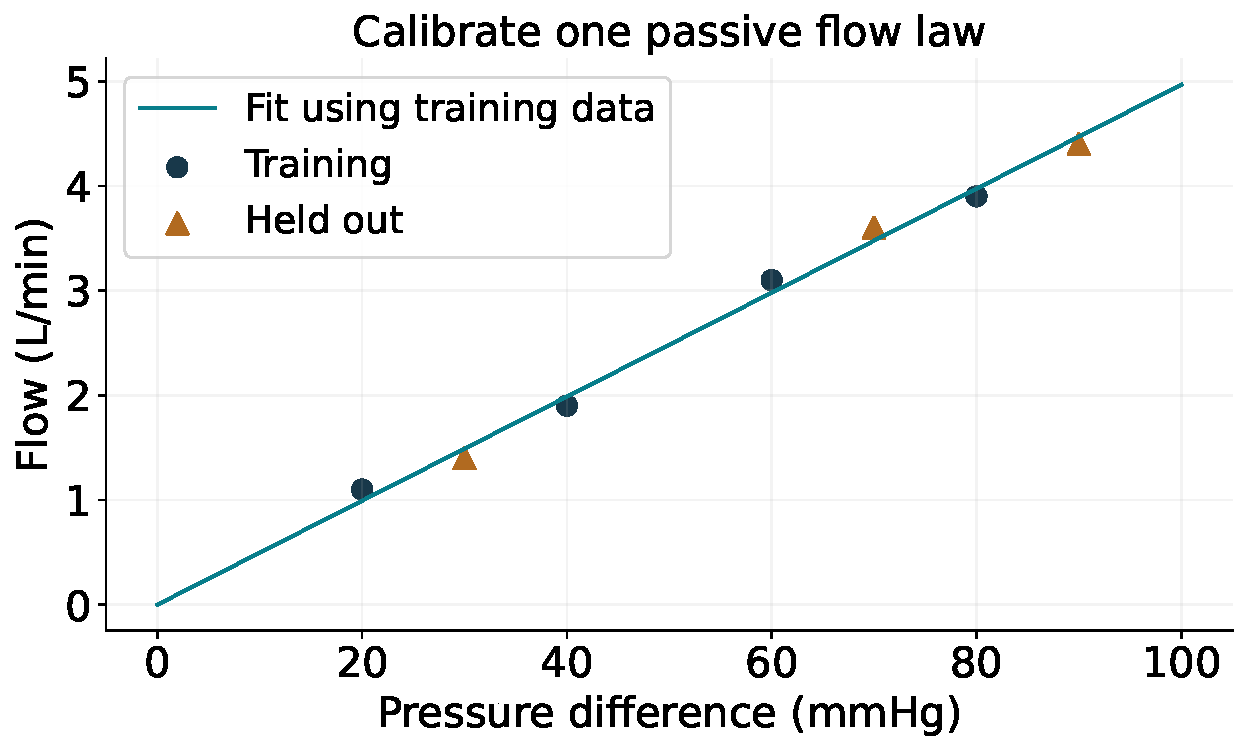
\includegraphics[width=.96\linewidth,height=.57\textheight,keepaspectratio]{calibration.pdf}\par\smallskip
{\small Synthetic training and held-out observations with a fitted through-origin law. The line predicts flow from a prescribed pressure difference; it does not simulate a complete circulation.}
\end{minipage}\end{center}
\section{Least squares without differentiation}
\hypertarget{note-least-squares-without-differentiation}{}\label{note:least-squares-without-differentiation}
{\small \href{slides.html\#frame=define-the-discrepancy\&step=1}{Slides for this section}}\par
Expand the square and collect the terms involving $G$:
\begin{equation}S(G)=AG^2-2BG+C,\qquad
A=\sum_{\mathcal T}x_i^2,\quad B=\sum_{\mathcal T}x_iy_i,\quad C=\sum_{\mathcal T}y_i^2.
\end{equation}
If $A>0$, completing the square gives
\begin{equation}S(G)=A\left(G-\frac BA\right)^2+C-\frac{B^2}{A}.\end{equation}
The second and third terms do not depend on $G$, and the squared term is nonnegative. Thus the unique unconstrained minimizer is
\begin{equation}\widehat G=\frac{\sum_{\mathcal T}x_iy_i}{\sum_{\mathcal T}x_i^2}.\label{eq:conductance-fit}\end{equation}
This argument uses only expansion and a nonnegative square. If every $x_i=0$, then $A=0$ and $S(G)=C$ for every conductance: the experiment contains no information about the slope. The companion additionally requires a positive fitted conductance before interpreting its reciprocal as resistance.

The four training pairs are $(20,1.1)$, $(40,1.9)$, $(60,3.1)$ and $(80,3.9)$ in the stated units. They give $A=12000$, $B=596$, and $\widehat G=596/12000\simeq0.049667$. Hence $\widehat R\simeq20.134\,\mathrm{mmHg\,min/L}$. The precision here reflects arithmetic on a synthetic dataset; it is not a precision claim about a measured vascular resistance.

There is also a useful unit check. If the numerical pressure values are replaced by $x'_i=cx_i$ with $c>0$, then $\widehat G'=\widehat G/c$. Consequently $\widehat G'x'_i=\widehat Gx_i$: the physical predictions are unchanged. A unit conversion changes the coefficient's numerical value and units together.
\section{A frozen rule on new observations}
\hypertarget{note-a-frozen-rule-on-new-observations}{}\label{note:a-frozen-rule-on-new-observations}
{\small \href{slides.html\#frame=evaluate-the-frozen-line\&step=1}{Slides for this section}}\par
The three held-out pairs are $(30,1.4)$, $(70,3.6)$ and $(90,4.4)$. Using the already selected conductance, their predictions are $1.4900$, $3.4767$ and $4.4700\,\mathrm{L/min}$. Their signed residuals are approximately $0.0900$, $-0.1233$ and $0.0700\,\mathrm{L/min}$. The mean absolute error is therefore
\begin{equation}\operatorname{MAE}=\frac{0.0900+0.1233+0.0700}{3}\simeq0.09444\,\mathrm{L/min}.
\end{equation}
Absolute error retains the unit of flow. Displaying the three residuals preserves information that their average loses, such as which pressure range has the largest error.

For a simple comparison, a predictor that always returns the training mean flow returns $2.5\,\mathrm{L/min}$. Its absolute errors on these same held-out points are $1.1$, $1.1$ and $1.9$, averaging $1.3667\,\mathrm{L/min}$. This comparison is additional arithmetic on the displayed observations, not a separate physiological model or a claim about a population. Three test observations provide a small check of prediction, not a reliable estimate of every future error.

If the held-out errors are used to choose a new offset or a new family of curves, the rows have become part of model development. Testing the revised rule requires other observations. The appropriate separation also depends on the intended claim: repeated measurements from one preparation do not automatically test performance on a new preparation.
\section{Training coordinates and class centers}
\hypertarget{note-training-coordinates-and-class-centers}{}\label{note:training-coordinates-and-class-centers}
{\small \href{slides.html\#frame=fit-a-coordinate-system-on-training-cases-figure\&step=1}{Slides for this section}}\par
The classification experiment has eighty synthetic cases with two features: a rate and a magnitude describing interval variation. Labels $0$ and $1$ identify two generator regimes, not diagnoses. Forty-eight cases define the model and thirty-two are held out. The generator clips both raw features below at a positive value, so these are explicitly constructed measurements rather than an unmodified Gaussian physiological model.

For feature $j$, compute a training mean $\mu_j$ and training standard deviation $s_j>0$, then use
\begin{equation}z_j=\frac{x_j-\mu_j}{s_j}.
\end{equation}
The same $\mu_j,s_j$ transform every future row. A standardized value of one means one training standard deviation above the training mean. It does not give the two physical measurements the same biological interpretation. For label $k$, average its standardized training rows to obtain a center $c_k$. Classify a new point by its smaller squared distance:
\begin{equation}\widehat k(z)=\mathop{\rm argmin}_{k\in\{0,1\}}\|z-c_k\|^2,
\qquad \|z-c_k\|^2=\sum_{j=1}^2(z_j-c_{kj})^2.
\end{equation}
The implementation assigns exact ties to label zero. Both feature scaling and the centers are fitted quantities. Computing the scale from all eighty rows would let the held-out cases alter the geometry used to classify themselves.
\begin{center}\begin{minipage}{.98\linewidth}\centering
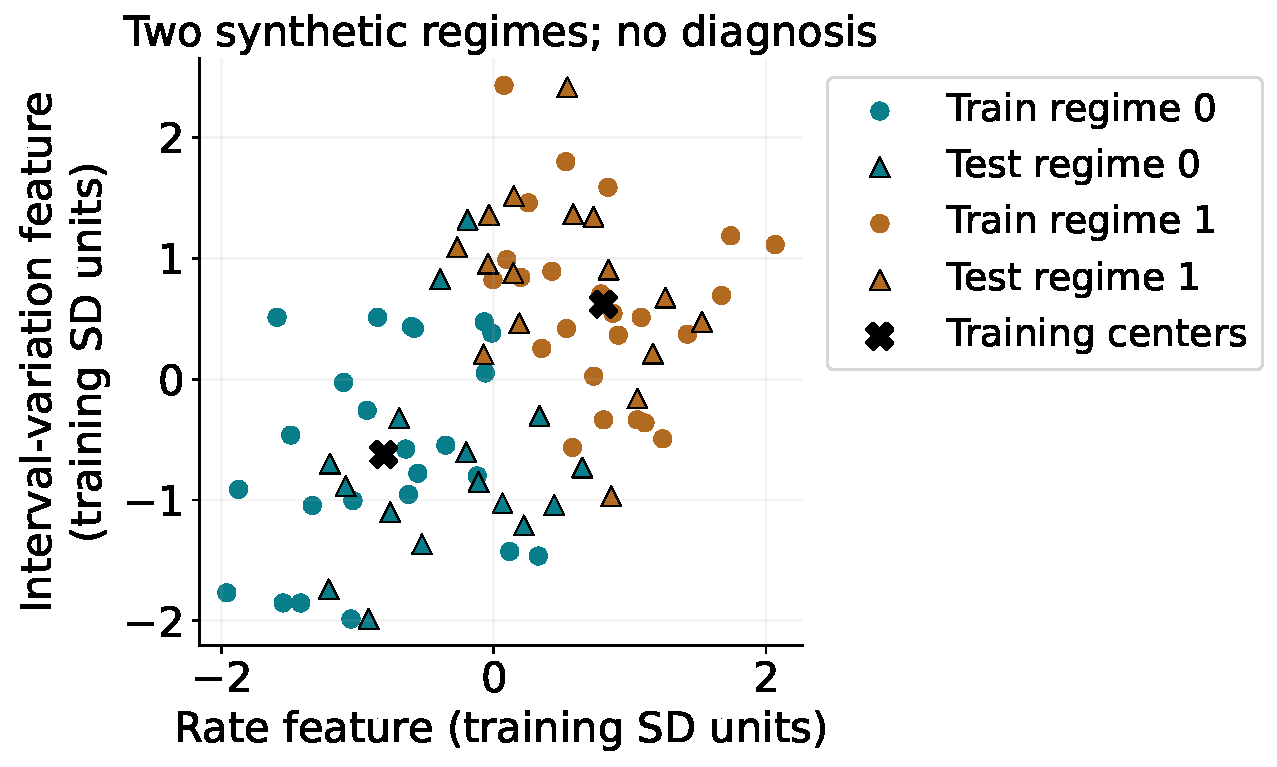
\includegraphics[width=.96\linewidth,height=.57\textheight,keepaspectratio]{classification.pdf}\par\smallskip
{\small Training means and scales define the axes; circles are training cases, triangles are held-out cases, and crosses are training centers. Generator regimes have no diagnostic interpretation.}
\end{minipage}\end{center}
\section{The boundary hidden in the distance comparison}
\hypertarget{note-the-boundary-hidden-in-the-distance-comparison}{}\label{note:the-boundary-hidden-in-the-distance-comparison}
{\small \href{slides.html\#frame=expand-the-decision-boundary\&step=1}{Slides for this section}}\par
The nearest-center rule has a simple geometry. Label one is chosen when $\|z-c_1\|^2<\|z-c_0\|^2$. Expanding both sides cancels $z_1^2+z_2^2$ and gives
\begin{equation}2z\mathbin{\cdot}(c_1-c_0)>\|c_1\|^2-\|c_0\|^2.\end{equation}
Equality describes a straight line in the two-dimensional standardized coordinates, provided the centers differ. Thus the apparently nonlinear squared-distance comparison defines a linear boundary. It cannot follow an arbitrary curved separation between classes.

Scaling changes that geometry in raw coordinates. If $\overline x_{kj}$ is the raw class mean, then
\[\|z-c_k\|^2=\sum_{j=1}^2\frac{(x_j-\overline x_{kj})^2}{s_j^2}.
\]
A feature with larger training variation receives smaller weight per squared raw-unit difference. This explains why changing units consistently need not change the classification, whereas deciding on a different scaling rule can. The decision also discards the distinction between points near and far from both centers: nearest does not necessarily mean close. No calibrated probability is produced by this rule.
\section{Count the errors the claim actually concerns}
\hypertarget{note-count-the-errors-the-claim-actually-concerns}{}\label{note:count-the-errors-the-claim-actually-concerns}
{\small \href{slides.html\#frame=read-both-directions-of-error\&step=1}{Slides for this section}}\par
With true labels as rows and predictions as columns, the held-out confusion table is
\[
\begin{array}{c|rr}
&\widehat k=0&\widehat k=1\\\hline
k=0&12&4\\
k=1&0&16
\end{array}
\]
There are $28$ correct predictions out of $32$, giving accuracy $0.875$. Of the $16$ true label-zero cases, $4$ are mislabeled one. Of the $16$ true label-one cases, none is mislabeled zero. The balanced test sample would give accuracy $0.5$ to either constant-label rule. These counts concern generator labels, so interpreting them as clinical sensitivity or specificity would change the meaning of the target.

For a claim about new people, splitting individual windows is inadequate when windows from the same person can enter both sets. The grouping unit must be the person; training transformations and centers must then use training people only. Even that split does not repair inaccurate labels or a population unlike the intended application. The mathematical rule is completely specified here, but the scientific claim still depends on how observations and labels were obtained.
\bigskip
\section*{Exercises}
\par\noindent\begin{minipage}{\linewidth}
\subsection*{MC08-E1. A small calibration}
Synthetic observations are (10 mmHg, 0.6 L/min) and (30 mmHg, 1.8 L/min).

\textbf{a} Compare squared-error totals for G=\allowbreak{}0.05 and 0.06 L/(min mmHg).

\end{minipage}\par\medskip
\textbf{b} Find resistance for the better candidate, with units.

\textbf{c} Explain why perfect fit is not validation.

\par\noindent\begin{minipage}{\linewidth}
\subsection*{MC08-E2. Test the frozen rule}
Freeze G=\allowbreak{}.04 L/(min mmHg). Held-out observations are (25 mmHg, 1.2 L/min) and (50 mmHg, 1.7 L/min).

\textbf{a} Calculate predictions, signed residuals predicted minus observed, and MAE.

\end{minipage}\par\medskip
\textbf{b} A colleague changes G after seeing these errors. What status do these rows now have, and how should the revised rule be evaluated?

\textbf{c} Name a useful additional test.

\par\noindent\begin{minipage}{\linewidth}
\subsection*{MC08-E3. Read a confusion table}
For 20 new synthetic cases: true 0/pred 0=\allowbreak{}7; true 0/pred 1=\allowbreak{}3; true 1/pred 0=\allowbreak{}2; true 1/pred 1=\allowbreak{}8.

\textbf{a} Compute accuracy and both error counts.

\end{minipage}\par\medskip
\textbf{b} Compute the fraction of true 1 cases detected as 1.

\textbf{c} Why does that fraction not establish clinical sensitivity?

\par\noindent\begin{minipage}{\linewidth}
\subsection*{MC08-E4. A project evaluation plan}
A project records five consecutive windows from each of ten volunteers. No data collection is required for this exercise.

\textbf{a} For a claim about new people, explain why randomly splitting windows is weak.

\end{minipage}\par\medskip
\textbf{b} Give a better split and specify when scaling is fitted.

\textbf{c} State one limitation that remains and explain how it affects the conclusion.

\section*{References}
\noindent\begin{minipage}{\linewidth}
Zan Ahmad, Mathematical Cardiology syllabus, Fall 2023. Public PDF pages 1--2, Course Topics and Course Objectives.

\url{https://zanahmad.com/files/Fall_2023_HEART_Syllabus.pdf}
\end{minipage}\par\medskip
\noindent\begin{minipage}{\linewidth}
Zan Ahmad, original editable Mathematical Cardiology syllabus. Rendered export pages 2--3, Assignments \& Grading and Projects.

\end{minipage}\par\medskip
\noindent\begin{minipage}{\linewidth}
Zan Ahmad, Introduction to Scientific Python, Lecture 5; source lineage includes Phillip Kerger (2023). PDF pages 5--12, learning tasks and linear regression.

\end{minipage}\par\medskip
\noindent\begin{minipage}{\linewidth}
scikit-learn, Common pitfalls and recommended practices. Sections 12.1 and 12.2, inconsistent preprocessing and data leakage; read 2026-11-14.

\url{https://scikit-learn.org/stable/common_pitfalls.html}
\end{minipage}\par\medskip
\end{document}
